\documentclass[12pt]{article}
\usepackage[paper=letterpaper,margin=2cm]{geometry}
\usepackage{amsmath}
\usepackage{amssymb}
\usepackage{amsfonts}
\usepackage{newtxtext, newtxmath}
\usepackage{enumitem}
\usepackage{titling}
\usepackage[colorlinks=true]{hyperref}
\usepackage{graphicx}
\usepackage{float}
\usepackage{listings}
\usepackage{xcolor}
\usepackage{color}
\definecolor{dkgreen}{rgb}{0,0.6,0}
\definecolor{gray}{rgb}{0.5,0.5,0.5}
\definecolor{mauve}{rgb}{0.58,0,0.82}
\lstset{ %
        language=Java,                
  basicstyle=\footnotesize,     
  numbers=left,               
  numberstyle=\tiny\color{gray},
  stepnumber=1,                                       
  numbersep=5pt,                 
  backgroundcolor=\color{white},  
  showspaces=false,             
  showstringspaces=false,         
  showtabs=false,                 
  frame=single,                   
  rulecolor=\color{black},       
  tabsize=4,                   
  captionpos=b,        
  breaklines=true,             
  breakatwhitespace=false,       
  title=\lstname,                                                  
  keywordstyle=\color{blue},          
  commentstyle=\color{dkgreen},    
  stringstyle=\color{mauve},       
  escapeinside={\%*}{*},        
  morekeywords={*,...}
} 

\setlength{\droptitle}{-6em}

% Enter the specific assignment number and topic of that assignment below, and replace "Your Name" with your actual name.
\title{Assignment 3: Comp 6771 Image Processing}
\author{Yunqi Xu 40130514}
\date{\today}



\begin{document}
% \maketitle

\begin{titlepage}
  \rule{\textwidth}{1pt}   % The top horizontal rule
    \vspace{0.2\textheight}  % Whitespace between top horizontal rule and title

    %------------------------------------------------------------
    %    Title
    %------------------------------------------------------------

    {\Huge COMP 6771 Image Processing: Assignment 2}

    \vspace{0.025\textheight}   % Whitespace between the title and short horizontal rule

    \rule{0.83\textwidth}{0.4pt}  % The short horizontal rule under title

    \vspace{0.1\textheight}  % Whitespace between the short horizontal rule and author

    %------------------------------------------------------------
    %    Author
    %------------------------------------------------------------

    {\Large Student name: \textsc{Yunqi Xu}}
    \vfill
    {\Large Student id: 40130514}
    \vfill  % Whitespace between author and date

    {\large \today}
    \vspace{0.1\textheight}  % Whitespace between date and bottom horizontal rule

    %------------------------------------------------------------
    %    Bottom rules
    %------------------------------------------------------------

    \rule{\textwidth}{1pt}  % The bottom horizontal rule
\end{titlepage}

\begin{enumerate}[leftmargin=\labelsep]
% \vspace*{40em}
\item Theoretical Question 1

    
    Based on the question, the mask is:
        \begin{equation}
            g(x, y) = \frac{1}{4}[f(x, y-1) + f(x, y+1) +f(x-1, y) +f(x+1, y)]  
            \label{q1_eq1}    
        \end{equation}
        Also, 
        \begin{equation}
            f(x - x_{0}, y - y_{0}) = F(u, v)e^{-j2 \pi (ux_{0}/M + vy_{0}/N)}
            \label{q1_eq2}
        \end{equation}

        Based on the Eq.~\ref{q1_eq2}, the Eq.~\ref{q1_eq1} can be calculated like:
        \begin{equation}
            \begin{aligned}
                f(x, y-1)
                &= f(x - 0, y -(1))\\
                &= F(u, v)e^{-j2\pi(u(0)/M + v(1)/N)}\\
                &= F(u, v)e^{-j2\pi v/N}
                \label{q1_eq3}
            \end{aligned}
        \end{equation}
        
        \begin{equation}
            \begin{aligned}
                f(x, y+1) 
                &= f(x-0, y-(-1))\\
                &= F(u, v)e^{-j2\pi (u(0)/M + v(-1)/N)}\\
                &= F(u, v)e^{j2\pi v/N}
            \label{q1_eq3}
            \end{aligned}
        \end{equation}

        \begin{equation}
            \begin{aligned}
                f(x-1, y) 
                &= f(x-(1), y-0)\\
                &= F(u, v)e^{-j2\pi(u(1)/M + v(0)/N)}\\
                &= F(u, v)e^{-j2\pi u/M}
            \label{q1_eq4}
            \end{aligned}
        \end{equation}

        \begin{equation}
            \begin{aligned}
                f(x+1, y) 
                &= f(x-(-1), y-0)\\
                &= F(u, v)e^{-j2\pi(u(-1)/M + v(0)/N)}\\
                &= F(u, v)e^{j2\pi u/M}
            \label{q1_eq5}
            \end{aligned}
        \end{equation}
        
        So, based on the Eq.~\ref{q1_eq2} ~\ref{q1_eq3} ~\ref{q1_eq4} ~\ref{q1_eq5}, 

        \begin{equation}
            G(u, v) = \frac{1}{4} F(u, v) [e^{-j2\pi v/N} + e^{j2\pi v/N} + e^{-j2\pi u/M} + e^{j2\pi u/M}]
        \end{equation}

        \begin{equation}
            H(u, v) = \frac{1}{4} [e^{-j2\pi v/N} + e^{j2\pi v/N} + e^{-j2\pi u/M} + e^{j2\pi u/M}]
        \end{equation}

        Based on the Euler's Formula, $\cos \theta = \frac{1}{2}(e^{i \theta} + e^{-i \theta})$,

        \begin{equation}
            \begin{aligned}
                H(u, v)
                &= \frac{1}{4}F(u, v)[2\cos(\frac{2 \pi v}{N} + 2\cos(\frac{2\pi u}{M}))]\\
                &= \frac{1}{2}F(u, v)[\cos(\frac{2 \pi v}{N} + \cos(\frac{2\pi u}{M}))]
            \end{aligned}
        \end{equation}

    \vspace*{7em}

\item Theoretical Question 2

\begin{enumerate}
    \item  If an equation is linear, which means that:
    \begin{equation}
        O(af_{1}(x, y) + bf_{2}(x, y)) = aO(f_{1}(x, y)) + bO(f_{2}(x, y))
        \label{q2_eq1}
    \end{equation}
    In Eq.~\ref{q2_eq1}, the $O()$ is an operator.
    So in this queation:
    \begin{equation}
        \begin{aligned}
        O(af_{1}(x, y) + bf_{2}(x, y))
        &= \int_{-\infty}^{\infty}\int_{-\infty}^{\infty}(af_1(x, y) + bf_2(x, y))\delta(x\cos\theta + y\sin\theta - \rho)dxdy\\
        &= a\int_{-\infty}^{\infty}\int_{-\infty}^{\infty}f_1(x, y)\delta(x\cos\theta + y\sin\theta - \rho)dxdy + \\
        & b\int_{-\infty}^{\infty}\int_{-\infty}^{\infty}f_2(x, y)\delta(x\cos\theta + y\sin\theta - \rho)dxdy\\
        &= aO(f_1(x, y)) + bO(f_2(x, y))
        % \label(q2_eq2)
        \end{aligned}
    \end{equation}
    So it is linear operator.

    \item Based on the priciple of Integral by substitution:
    \begin{equation}
     \begin{aligned}
        u = x - x_0\\
        v = y - y_0
        \end{aligned}
    \end{equation}

    \begin{equation}
        \begin{aligned}
            x = u + x_0\\
            y = v + y_0
        \end{aligned}
    \end{equation}

    \begin{equation}
        \begin{aligned}
            du = dx \\
            dv = dy
        \end{aligned}
    \end{equation}

    So, 
    \begin{equation}
        \begin{aligned}
                f(\rho, \theta)
                &= \int_{-\infty}^{\infty}\int_{-\infty}^{\infty}f(x - x_0, y - y_0) \delta(x\cos\theta + y\sin\theta - \rho)dxdy\\
                &= \int_{-\infty}^{\infty}\int_{-\infty}^{\infty}f(u, v)\delta[(u + x_0)\cos\theta + (v + y_0)\sin\theta - \rho)dudv\\
                &= \int_{-\infty}^{\infty}\int_{-\infty}^{\infty}f(u, v)\delta(u\cos\theta + x_0\cos\theta + v\sin\theta + y_0\sin\theta - \rho)dudv\\
                &= \int_{-\infty}^{\infty}\int_{-\infty}^{\infty}f(u, v)\delta(u\cos\theta + v\sin\theta - (\rho - x_0\cos\theta - y_0\sin\theta))dudv\\
                &= g(\rho - x_0\cos\theta - y_0\sin\theta, \theta)
        \end{aligned}
    \end{equation}    

\end{enumerate}

\item Programming Question 1 
\begin{enumerate}
\item The code is shown blow.
\begin{lstlisting}
    %read image
    img_house = imread("house.tif");
    img_jet = imread("jet.tiff");
    img_house = img_house(:, :, 1);
    img_jet = img_jet(:, :, 1);
    
    
    % Fourier Transformer
    img_house_f = fft2(double(img_house));
    img_jet_f = fft2(double(img_jet));
    
    %calculate the magnitude and phase of house
    img_house_m = abs(img_house_f);
    img_house_ph = angle(img_house_f);
    
    %calculate the magnitude and phase of jet
    img_jet_m = abs(img_jet_f);
    img_jet_ph = angle(img_jet_f); 
    
    %reconstruct images
    image_a=img_house_m.*cos(img_jet_ph)+img_house_m.*sin(img_jet_ph).*1i;
    image_b=img_jet_m.*cos(img_house_ph)+img_jet_m.*sin(img_house_ph).*1i;
    image_a=abs(ifft2(image_a));
    image_b=abs(ifft2(image_b));
    image_a=uint8(image_a);
    image_b=uint8(image_b);
    
    
    % plot images
    subplot(2,2,1);imshow(img_house);title('House');
    subplot(2,2,2);imshow(img_jet);title('Jet');
    subplot(2,2,3);imshow(image_a);title('Magenitude of house with phase of Jet');
    subplot(2,2,4);imshow(image_b);title('Magnitude of Jet with phase of House');
\end{lstlisting}

The images are shown below:
\begin{figure}[H]
    \centering
    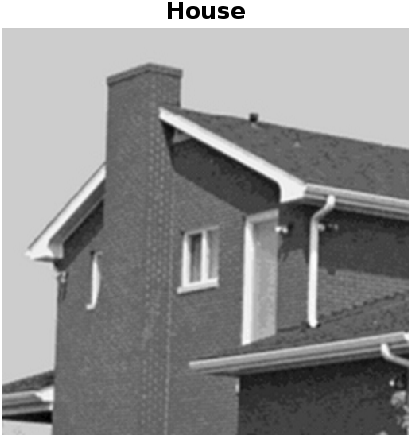
\includegraphics[]{Figure/House.png}
    \caption{Input House}
    \label{Q3_1}
\end{figure}

\begin{figure}[H]
    \centering
    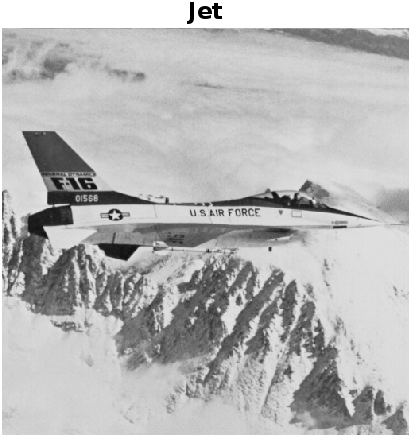
\includegraphics[]{Figure/Jet.png}
    \caption{Input Jet}
    \label{Q3_2}
\end{figure}

\begin{figure}[H]
    \centering
    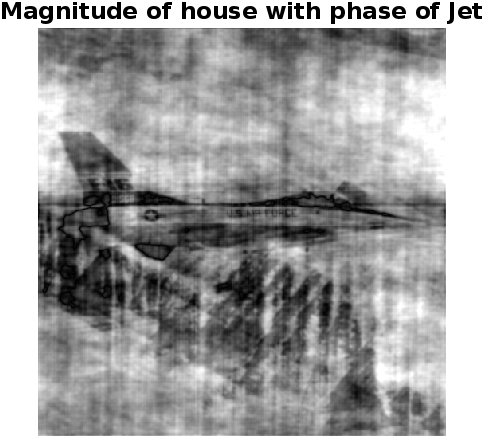
\includegraphics[]{Figure/Magnitude of house with phase of Jet.png}
    \caption{Magnitude of house + phase of Jet}
    \label{Q3_3}
\end{figure}

\begin{figure}[H]
    \centering
    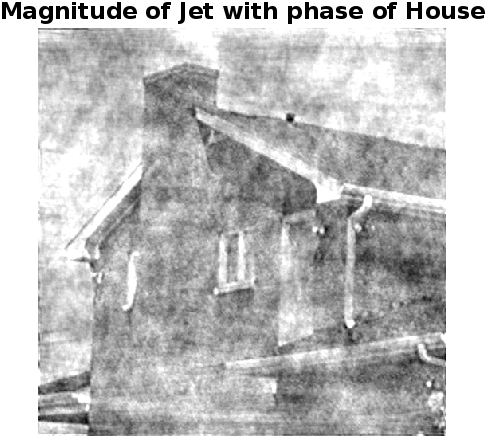
\includegraphics[]{Figure/Magnitude of Jet with phase of House.png}
    \caption{Magnitude of Jet + phase of House}
    \label{Q3_4}
\end{figure}

Suppose the Fig.~\ref{Q3_1} (House) is $I_A$, so the Fig.~\ref{Q3_4}(Magnitude of Jet with Phase of House) is the better construction.
On the other hand, suppose the Fig.~\ref{Q3_2} (Jet) is $I_A$, then the Fig.~\ref{Q3_3}(Magnitude of House with Phase of Jet) is the better construction.
The Fig.~\ref{Q3_3} and Fig.~\ref{Q3_4} indicates that for reconstruction, the phase of an image usually contains more edge and strcture information. So the Fig.~\ref{Q3_3} has a jet, and Fig.~\ref{Q3_4} has a house.

\end{enumerate}


\item Programming Q2
\begin{enumerate}
    \item The code is shown below
    \begin{lstlisting}
def readImg(path):
return cv.imread(path, 0)

def gaussianBlur(img = None, kernal_size = None, sigma = None):
    return cv.GaussianBlur(img, (kernal_size, kernal_size), sigma)

def laplacian(img = None, kernal_size = None):
    return cv.Laplacian(img, cv.CV_16S, ksize = kernal_size)

def zero_cross(input_image = None, threshold = None):
    zero_cross = np.zeros_like(input_image, dtype=np.uint8)
    image_height, image_width = input_image.shape
    for y in range(1, image_height - 1):
        for x in range(1, image_width - 1):
            if input_image[y][x] == 0:
                if input_image[y][x - 1] * input_image[y][x + 1] < 0:
                    if np.abs(input_image[y][x - 1] - input_image[y][x + 1]) / 2 > threshold:
                        zero_cross[y][x] = 255

                if input_image[y - 1][x] * input_image[y + 1][x] < 0:
                    if np.abs(input_image[y - 1][x] - input_image[y + 1][x]) / 2 > threshold:
                        zero_cross[y][x] = 255

                if input_image[y - 1][x - 1] * input_image[y + 1][x + 1] < 0:
                    if np.abs(input_image[y - 1][x - 1] - input_image[y + 1][x + 1]) / 2 > threshold:
                        zero_cross[y][x] = 255

                if input_image[y - 1][x + 1] * input_image[y + 1][x - 1] < 0:
                    if np.abs(input_image[y - 1][x + 1] - input_image[y + 1][x - 1]) / 2 > threshold:
                        zero_cross[y][x] = 255
            if input_image[y][x] < 0:
                if (input_image[y][x - 1] > 0) or (input_image[y][x + 1] > 0) or \
                        (input_image[y - 1][x] > 0) or (input_image[y + 1][x] > 0) or \
                        (input_image[y - 1][x - 1] > 0) or (input_image[y + 1][x + 1] > 0) or \
                        (input_image[y - 1][x + 1] > 0) or (input_image[y + 1][x - 1] > 0):
                    if np.abs(input_image[y][x - 1] - input_image[y][x]) > threshold or \
                            np.abs(input_image[y][x + 1] - input_image[y][x]) > threshold or \
                            np.abs(input_image[y - 1][x] - input_image[y][x]) > threshold or \
                            np.abs(input_image[y + 1][x] - input_image[y][x]) > threshold or \
                            np.abs(input_image[y - 1][x - 1] - input_image[y][x]) > threshold or \
                            np.abs(input_image[y + 1][x - 1] - input_image[y][x]) > threshold or \
                            np.abs(input_image[y - 1][x + 1] - input_image[y][x]) > threshold or \
                            np.abs(input_image[y + 1][x + 1] - input_image[y][x]) > threshold:
                        zero_cross[y][x] = 255
    return zero_cross

def round_up_to_odd(f):
    return int(np.ceil(f) // 2 * 2 + 1)


def marrHildreth():
    # read image
    img = readImg("house.tif")
    # Gaussian blur

    gaussian_sigma = 3.7
    gaussian_kernal_size = round_up_to_odd(gaussian_sigma * 6)
    print(gaussian_kernal_size)
    img_gaussian = gaussianBlur(img=img,kernal_size=gaussian_kernal_size, sigma=gaussian_sigma)
    cv.imshow("gaussianblur", img_gaussian)

    # laplacian
    log_size= 9
    img_log = laplacian(img = img_gaussian, kernal_size= log_size)
    # zero crossing
    threshold = np.max(img_log) * 0.25
    img_zerocross = zero_cross(input_image=img_log, threshold=threshold)

    cv.imshow("marrHildreth", img_zerocross)
    cv.waitKey(0)
    cv.destroyAllWindows()

    marrHildreth()

    def canny():
    # read image
    img = readImg("house.tif")

    # Gauss blur
    gaussian_sigma = 1.5
    gaussian_kernal_size = round_up_to_odd(gaussian_sigma * 6)
    print(gaussian_kernal_size)
    img_gaussian = gaussianBlur(img=img,kernal_size=gaussian_kernal_size, sigma=gaussian_sigma)

    # Canny
    img_min = np.min(img_gaussian)
    img_max = np.max(img_gaussian)
    print((img_min, img_max))
    max_threshold = img_max * 0.6
    min_threshold = img_max * 0.2
    print((min_threshold, max_threshold))
    img_can = cv.Canny(img_gaussian, min_threshold, max_threshold)

    cv.imshow("canny", img_can)
    cv.waitKey(0)
    cv.destroyAllWindows()

    canny()
    \end{lstlisting}
     The code above indicates the details of implement the Marr-Hildreth and Canny edge detector.
    \begin{enumerate}
        \item In the implement of Marr-Hildreth, first, read the image into gray image, then use Gaussian Blur to blur the image for reducing noises, then use the Laplacian to find edges, finally use zero-crossing method to find more precise edges.
        \item In the Canny, first, read the image into gray image, then use Gaussian Blur to blur the image, reduce some noise, then use the Canny to filter the image. Also, the step inside Canny algorithm includes use Sobel operator find the magnitude and direction of edges, relate edge directions, non-maxmum suppression, and the detect edges and link edges.
    \end{enumerate}
    
    \item The edge linking in Canny algorithm includes, first give two threshold, a minimum one and maximum one. 
          After non-maxmum suppression, if the value of a pixel greater than the maximum threahold, this point will be treated as strong edge.
          On the other hand, if the value of a pixel smaller than the minimum threshold, this point is non-edge.
          Also, if the value of a pixel in the middle of the two threshold, this point will is weak edge. Then use 8-connectivity to detect whether this point belongs to a edge or not. 
          If this point connected with strong point, then it is belongs to edge otherwise not a point of edge.

          The edge linking step is not part of the step in Marr-Hildreth algorithm, cause Marr-Hildreth use zero-crossing method that based on the result of the Laplacian to find the edge. 
          In the code, the function zero\_cross() shows the details of zero-crossing method in Marr-Hildreth.
          Compared with the edge linking in Canny algorithm, the zero crossing in Marr-Hildreth will find those pixels which cross zero by detecting signs of its 8 neighbors and meanwhile checking the threshold between its neighbors for precise edges. 

    \item The parameters includes:
    \begin{enumerate}
        \item Marr-hildreth edge detector
            
        During the Gaussian blur process, we want gaussian blur small noises but keep more information of edges. In the image, the texture on the wall are some detail information need to be blured. 
        so we set $gaussian\_sigma = 3.7$ and the $gaussian\_size = max odd(6 * gaussian\_sigma) = 23$.  
        This parameters of Gaussian blur can fit the patterns in image, blur more small patterns and keep more inforamtion of edges.

        In the Laplacian filter process, we set $kernel\_size = 9$ in our experiment, this kernel size can fit the patterns of edges and give a good result for furthe step.

        During the zero crossing process, we set $threshold = max(laplacion\_result) * 0.25$ in our experiment. 
        Using this threshold, we can keep the most information of edges and remove as much non-edge information as we can.

        \item Canny edge detector
        
        Since the canny edge detector, since canny edge detector utilize non-maximum supression and edge linking to delete noise part. 
        So, during the Gaussian blur process, we set $gaussian\_sigma = 1.5$ and the $gaussian\_size = max odd(6 * gaussian\_sigma) = 9$ in our experiment. 
        This parameters can provide us a more clear information of edges.

        During the edge linking process, we set $max\_threshold = max value(img) * 0.6$ and $min\_threshold = max value(img) * 0.2$ in our experiment, and the $max\_threshold = 50$ and the $min\_threshold = 150$ during our calculate. 
        Also, the $max\_threshold / $min\_thresold$ = 150/50 = 3/1$ also following the rules for setting threshold.        
            
    \end{enumerate}
    


    \item 

        \begin{figure}[H]
            \centering
            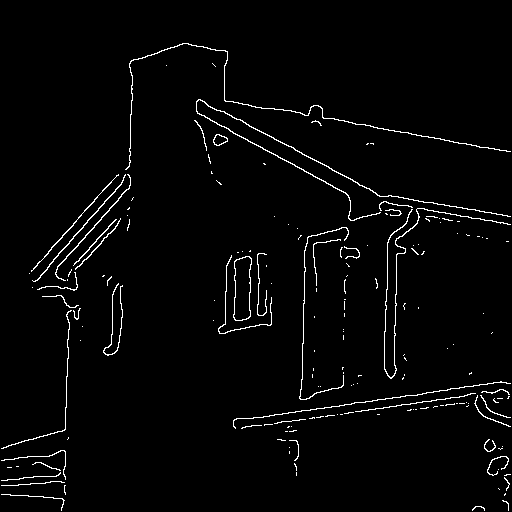
\includegraphics[width=0.5\textwidth,height=0.5\textwidth]{Figure/marrHildreth.png}
            \caption{The Marr-Hildreth result}
            \label{Q4_1}
        \end{figure}
        
        \begin{figure}[H]
            \centering
            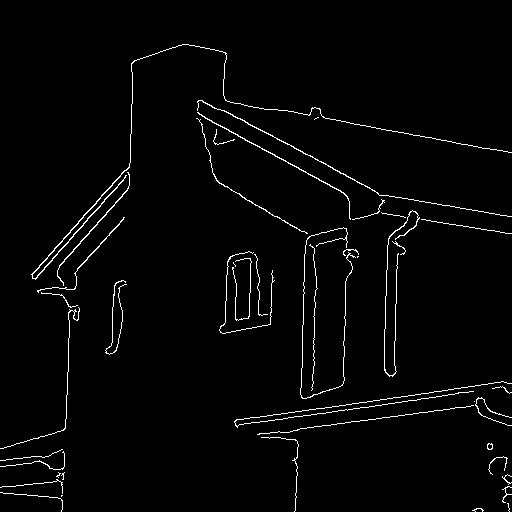
\includegraphics[width=0.5\textwidth,height=0.5\textwidth]{Figure/Canny.png}
            \caption{The Canny result}
            \label{Q4_2}
        \end{figure}

        The Fig.~\ref{Q4_1} and Fig.~\ref{Q4_2} present the result of these two edge detection algorithms. 
        Both of this two algorithm can detect the main edge.
        However, the edges in Fig.~\ref{Q4_2}(Canny edge detection) is better compared with the edges in Fig.~\ref{Q4_1}(Marr-Hildreth edge detection). 

        In Fig.~\ref{Q4_1}, there are some small noises which can not be removed since the restriction of the algorithm. 
        Since the threshold decide which pixels can be keeped can which pixels should be removed during the zero crossing process.
        This method may keep some pixels actually is noise but the intensity change are dramatical, even remove some pixels that actually belong to the edge.

        On the other hand, Canny algorithm can remains the correct edge information and remove those noises part in the image. Since the Non-maximum supression can delete many noise, and then the edge linking step further delete those pixels which are not edge points.
        

\end{enumerate}

\end{enumerate}

\end{document}
